\documentclass{article}

\usepackage{ amsmath, amssymb}
\usepackage{esvect}
\usepackage{bm}

% Tables.
\usepackage{multirow}
\usepackage{booktabs}

% Figures.
\usepackage{graphicx}
\graphicspath{{figures/}}
\usepackage{caption}
\usepackage{subcaption}
\usepackage{adjustbox}

% Citation/Bibliograph.
\usepackage{natbib} % Include `\cite` command.

\usepackage{hyperref}

% Symbols
\newcommand*\Laplace{\mathop{}\!\mathbin\bigtriangleup}
\newcommand*\DAlambert{\mathop{}\!\mathbin\Box}


\title{AM254 Final Paper}
\author{Noah Toyonaga}
\date{12/15/22}

\begin{document}
\maketitle


\section{Introduction}
Deriving the normal modes of a chain of masses connected by harmonic springs is one of the 
classic problems encountered in an introductory physics curriculum.
This exercise demonstrates the elegance of 
vector/matrix notations for coupled differential equations 
and simultanously motivates the connection between discrete and continuum systems. 
This project proceeds from this classic (and classical) system
and examines what happens when we augment or replace the nearest neighbor interactions with random couplings. 
The experiments which we will explore in this work are chosen to explore two regimes of geometric disorder. 
First, in which disorder is local, but strong (compared to the mean field/nearest neighbor model), and second in which disorder is long range but perturbative. 

\begin{enumerate}
	\item \textbf{Intermediate range}: We replace nearest neighbor interactions with random strength couplings to
		neighbors within a given bandwidth. 
		This corresponds to a graph laplacian with the approximate structure of band random matrices. 
	\item \textbf{Long range}: We assume and underlying nearest neighbor interaction but perturb the system with arbitrarily long range interactions.
		In particular, we compare the behaviour of the system in the presence of long range coupling to the behavior in the finite bandwidth regime. 
\end{enumerate}

We note that the above experiments do not represent an exhaustive typology of sources of disorder in a 1D lattice model. 
Freeman Dysons's first engagement with random matrix theory, for example,
was motivated by his investigation of the spectra 
of 1D lattices in which either the stiffness of the springs or mass of nodes are varied (\cite{Dyson1953-oa,Forrester2021-xr}). 

\subsection{The ordered chain and its spectrum.}

To eluciadate the random connection models, we first review the spring-lattice model and provide a construction 
for the stiffness matrix K.
Consider the 1D chain shown in fig. \ref{fig:1D_chain} which consists of $N$ masses (labeled $m_i$) and connecting springs (where a spring between $m_i$ and $m_j$ has a stiffness $k_{i,j}$).
The force experienced by the mass $m_i$ in the deformed configuration is given by the sum of forces due to adjacent springs as given by eq \ref{eq:general_lattice_force}.

\begin{equation}\label{eq:general_lattice_force}
\begin{split}
	f_i = k_{i,i+1}&\left[ \left(x_{i+1} + u_{i+1} \right)- \left(x_{i} + u_{i} \right)  - l_i\right] \\
		 &+ k_{i-1,i}\left[ \left(x_{i-1} + u_{i-1} \right)- \left(x_{i} + u_{i} \right)  - l_{i-1}\right]
\end{split}
\end{equation}


If we assume that the system is initally in an unstressed state 
(i.e. for every $i$, $x_{i+1} - x_{i} = l_i$) then \ref{eq:general_lattice_force} simplifies to:

\begin{equation}\label{eq:lattice_force}
	f_i = k_{i,i+1}\left[u_{i+1} - u_i\right] + k_{i-1, i}\left[u_{i-1} - u_{i}\right]
\end{equation}

We finally note that the $N$ system of equations corresponding to all the masses in the system can be concisely expressed by a linear equation \ref{eq:lattice_matrix}.
Here, the $i$-th element of $\bm{F}$ and $\bm{u}$ are the force on and displacement of the mass $m_i$ respectively.
The stiffness matrix $\bm{K}_0$ is given explicitly by \ref{eq:k_lattice}.

\textbf{Physical problem and normalizion:} For an interial system $F=ma=mu_{tt}$, so we can construct an eigenproblem from \ref{eq:lattice_matrix} whose solutions give the 
vibrational spectrum of the mass chain. 
We normalize the matrix $\bm{K}_0$ by a factor $\left(\frac{l}{N}\right)^{-2}$ so that it can be interpreted as the discrete spatial laplacian $\Laplace$ for a domain of size $l$. 
We further assume that a unit mass $m=1$ is distributed evenly over a total domain of size $l=1$.
In this problem $k_{i,j} = N$ so the total system has a stiffness equivalent to a single spring of stiffness $k=1$.

\begin{equation}\label{eq:lattice_matrix}
	\bm{F} = \bm{K}_0\bm{u} 
\end{equation}

\begin{equation}\label{eq:k_lattice}
		\bm{K}_0 = 
\begin{pmatrix}
	-(k_{0,1} + k_{1,2}) & k_{1,2} & 0 & &\cdots & 0 \\
	k_{1,2} & -(k_{1,2} + k_{2,3}) & k_{2,3} & 0 & \cdots & 0 \\
	\vdots & &\ddots& \ddots  & \ddots & 0\\
	0& & \cdots && -(k_{N-2, N-1} + k_{N-1, N}) & k_{N-1, N}\\
	0 & & \cdots & & k_{N-1, N}& -(k_{N-1, N} + k_{N, N+1})
\end{pmatrix} 
\end{equation}

Anticipating the addition of other non-adjacent bonds, we define a more general stiffness matrix $\bm{K}$ in \ref{eq:K_general}. 
We note that $\bm{K}$ is a generalized graph laplacian of the system weighted by the relevant spring stiffnesses (\cite{Chung1997-dc}).

\begin{equation}\label{eq:K_general}
	K_{i,j}= \begin{cases}
		-1 * \sum k_{i,j} & if i=j \\
		k_{i,j} & if i
	\end{cases}
\end{equation}

The frequency spectrum $\omega(M)^2 \equiv \lambda$ (where $M$ indexes the eigenmodes of $\bm{K}_0$) are illustrated in \ref{fig:lattice_spectrum}. 
We note that the $\omega(M)$ has a nonlinear dependence on $M$ for $M\gtrapprox N$.
This is an effect of the finite size of the system.

\begin{figure}
\begin{center}
	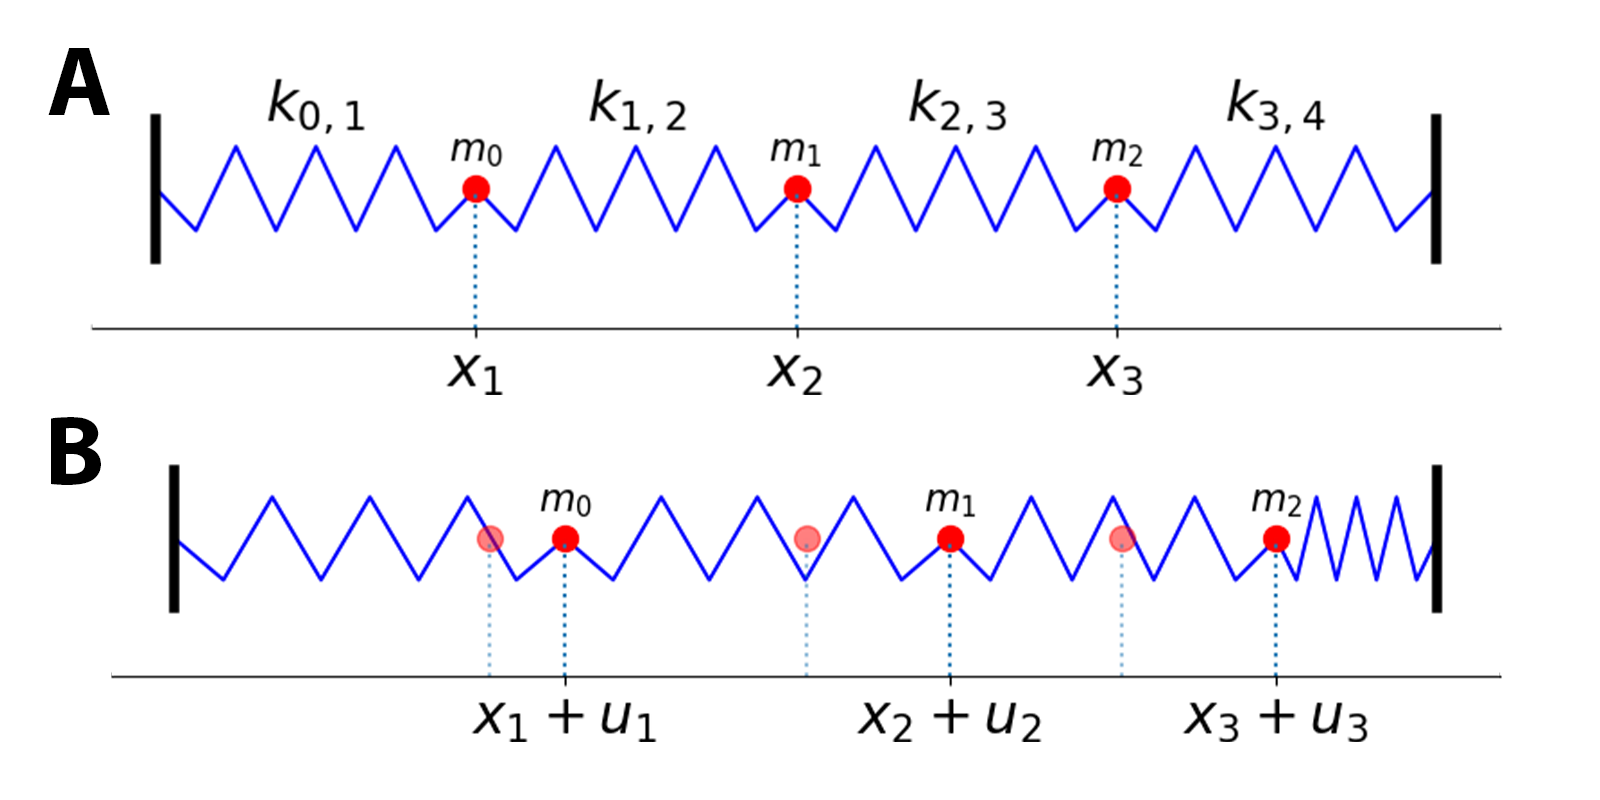
\includegraphics[width=.7\textwidth]{Figures/array.png}
\end{center}
\caption{A visual representation of a 1D chain with $N=3$ free nodes. 
	A. shows the (unstressed) equilibrium configuration while B. illustrates the deformed system.
The masses $m_i$ are indexed by $i \in (1, N)$, with corresponding displacements are $u_i$.}
\label{fig:1D_chain}
\end{figure}


\begin{figure}
\begin{center}
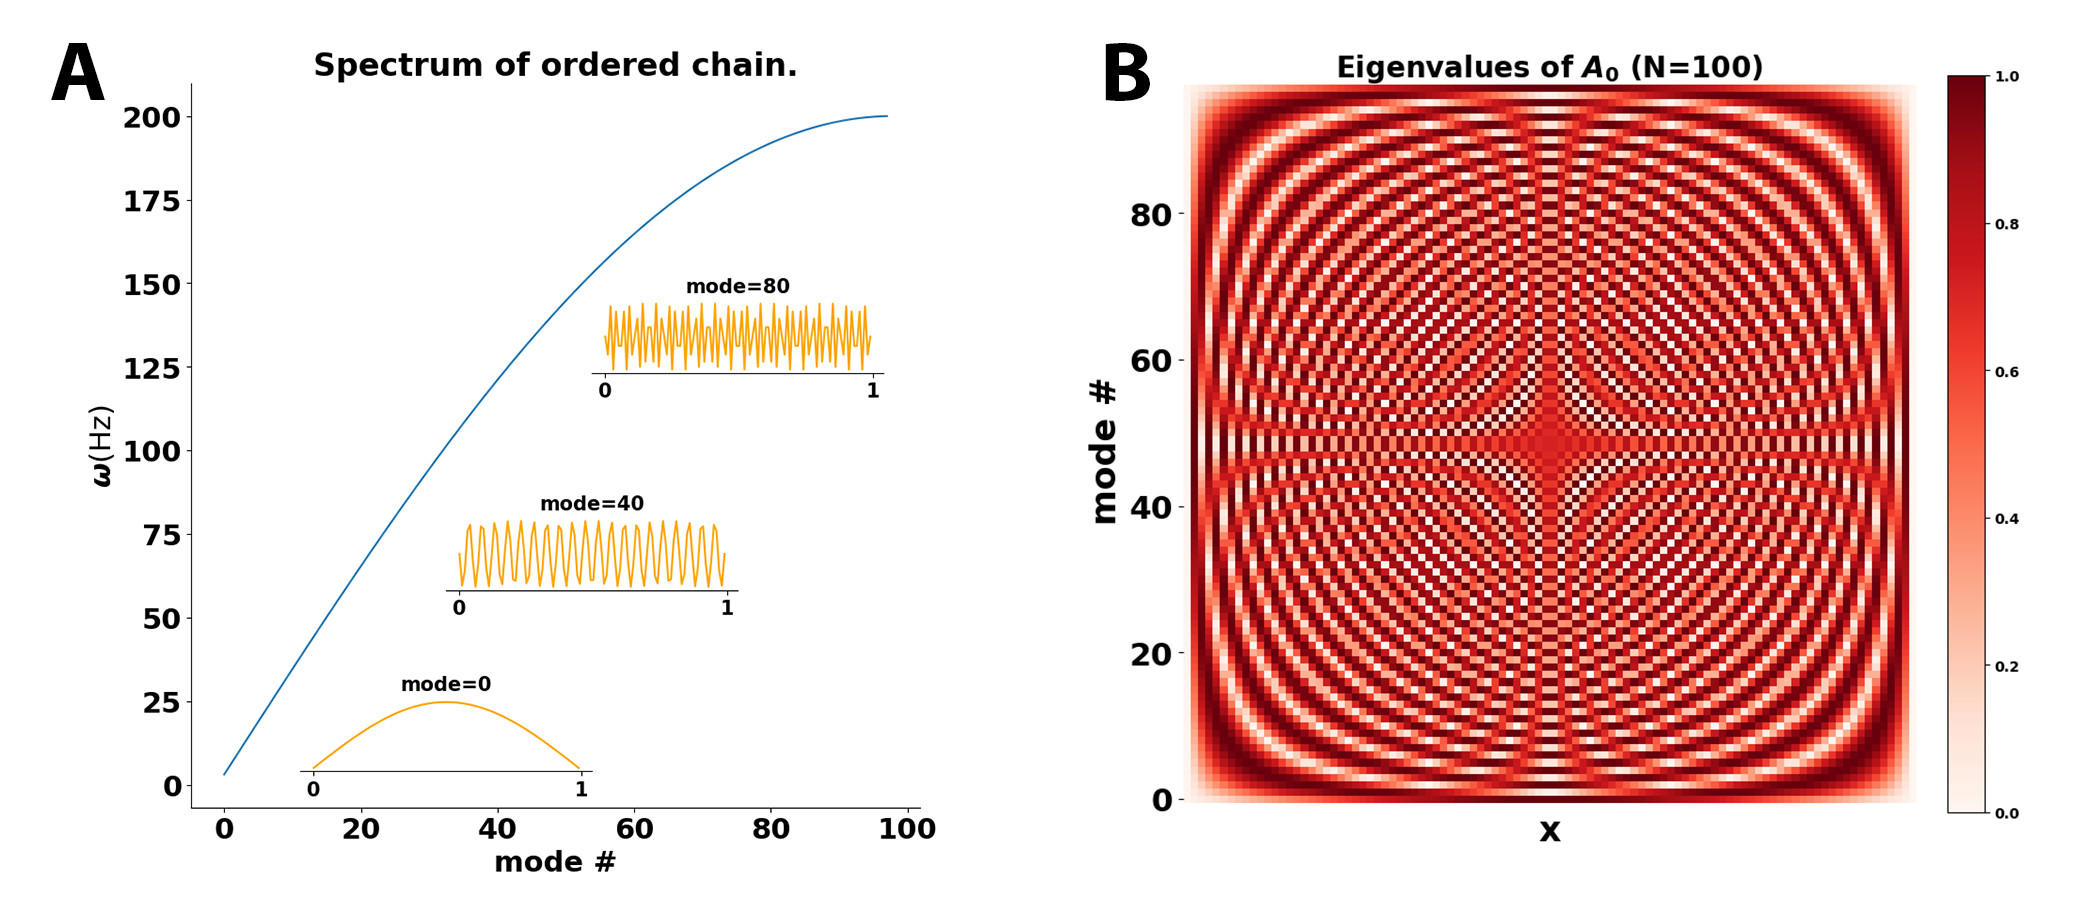
\includegraphics[width=\textwidth]{Figures/ordered_spectrum_and_eigenvector.png}
\end{center}
\caption{
	\textbf{A}. The spectrum of the 1D chain with stiffness matrix $\bm{K}_0$. 
	Inset plots show the eigenmodes corresponding to a given mode and frequency.
	We note that the mode $M=N$ corresponds to a bandwidth-limited signal for a signal sampled at a rate $1/N$. 
	\textbf{B}. The amplitude of the complete set of eigenmodes of the system, ordered from low to high frequency. 
Each row represents a single eigenmode.
We plot the absolute amplitude, rather than the signed aplitude in order to highlight the degree of (de)localization. 
Indeed, in the $\bm{K}_0$ system there are no localized modes in the sense defined in \ref{sec:localization}.}
\label{fig:lattice_spectrum}
\end{figure}

\section{Localization}
\label{sec:localization}

To motivate a study of eigenmode localization, we first consider the case of \textit{Anderson localization}, 
which correspoinds to the confinement of waves in the presence of a disordered background potential (\cite{Anderson1958-dt}).
This phenomena is of interest, because it suggests that evergy can be localized in a system without confinement.
While Anderson was specifically interested in localization of a quantum wavefunction on a disordered lattice, 
the phenomena holds for any system whose evolution is given by an elliptic operator.\footnote{
\cite{Filoche2012-av} give an elegant proof for the localization of eigenmodes as a conequence of a set of effective contraints defined in the \textit{interior} of the domain generated by the field $V$.}
The eigenproblem for this model is given by eq \ref{eq:anderson} where the potential $V(x)$ is a random distribution over space. 

\begin{equation}\label{eq:anderson}
	\left( -\Laplace + V\right)u = \lambda u 
\end{equation}

In our experiment, we construct $V$ by partitioning the domain into (n=20) bins and setting $V$ within each bin to a random value uniformly distribitued between $(0, N^2)$. 
A representative experiment is shown in \ref{fig:anderson_eigenvalues} were we can clearly see the spatial localization of eigenmodes in \ref{fig:anderson_eigenvalues}.C.

We observe in fig \ref{fig:anderson_eigenvalues}.A that the presence of the background field effectively 
rectifies the nonlinearity observed in the energy/frequency spectrum of the ordered lattice.
At the same time, there appears to be anomalous confinement of \textit{high} energy modes, 
which according to a continuum treatment should be fully delocalized (\cite{Filoche2012-av}).
Understanding the quasi-symmetry between the low energy and high energy confinement in this system may be 
of interest for future study.

\textbf{Localization Measurement} We now introduce two metrics for the degree of localization. 
The first, given by eq \ref{eq:localization_metric} was inspired by (\cite{Casati1990-ma}) and their study of
localization in the spectra of random band matrices. 
Roughly, \ref{eq:localization_metric_ind} corresponds to the information entropy of the eigenvector $u_i$ and small values
correspond to the intuitive idea of localization, that the eigenvector takes on small values everywhere except a restricted subset of the full domain.
Using $H$ we can also compute an average localization over a sample of eigenvectors $\Omega$.
In particular we will compute an average compared to a fully delocalized mode (corresponding to the eigenvectors of a GOE matrix).
In \cite{Casati1990-ma}, the authors show that the entropy of a GOE eigenvector takes an average value of $\Psi \left( 1/2 N + 1 \right) - \Psi \left( 3/2 \right)$
where $\Phi$ is the digamma function.


The second localization metric is simply the variance $\sigma^2$ of eigenvector, considered as a probability distribution.
In doing so, we of course limit our consideration to eigenvalues which localize in unimodal distributions, which may not be applicable for all interesting types of localization.
Even so, the strong localization exhibited e.g. by $M=0$ in fig \ref{fig:anderson_eigenvalues}.A inset will be captured by
the variance, even though it has a bimodal structure. 

We compare these two localization metrics for the anderson and ordered-chain models in fig \ref{fig:anderson_localization}.

\begin{subequations}
	\begin{equation}\label{eq:localization_metric_ind}
	H \left( u \right)\equiv \sum u_i ^2 \log{\left( u_i^2 \right)}
\end{equation}
\begin{equation}
	\beta \equiv \exp{\left( \langle H \rangle_\Omega - H_{GOE} \right)}
\end{equation}
\label{eq:localization_metric}
\end{subequations}

\begin{figure}
	\begin{center}
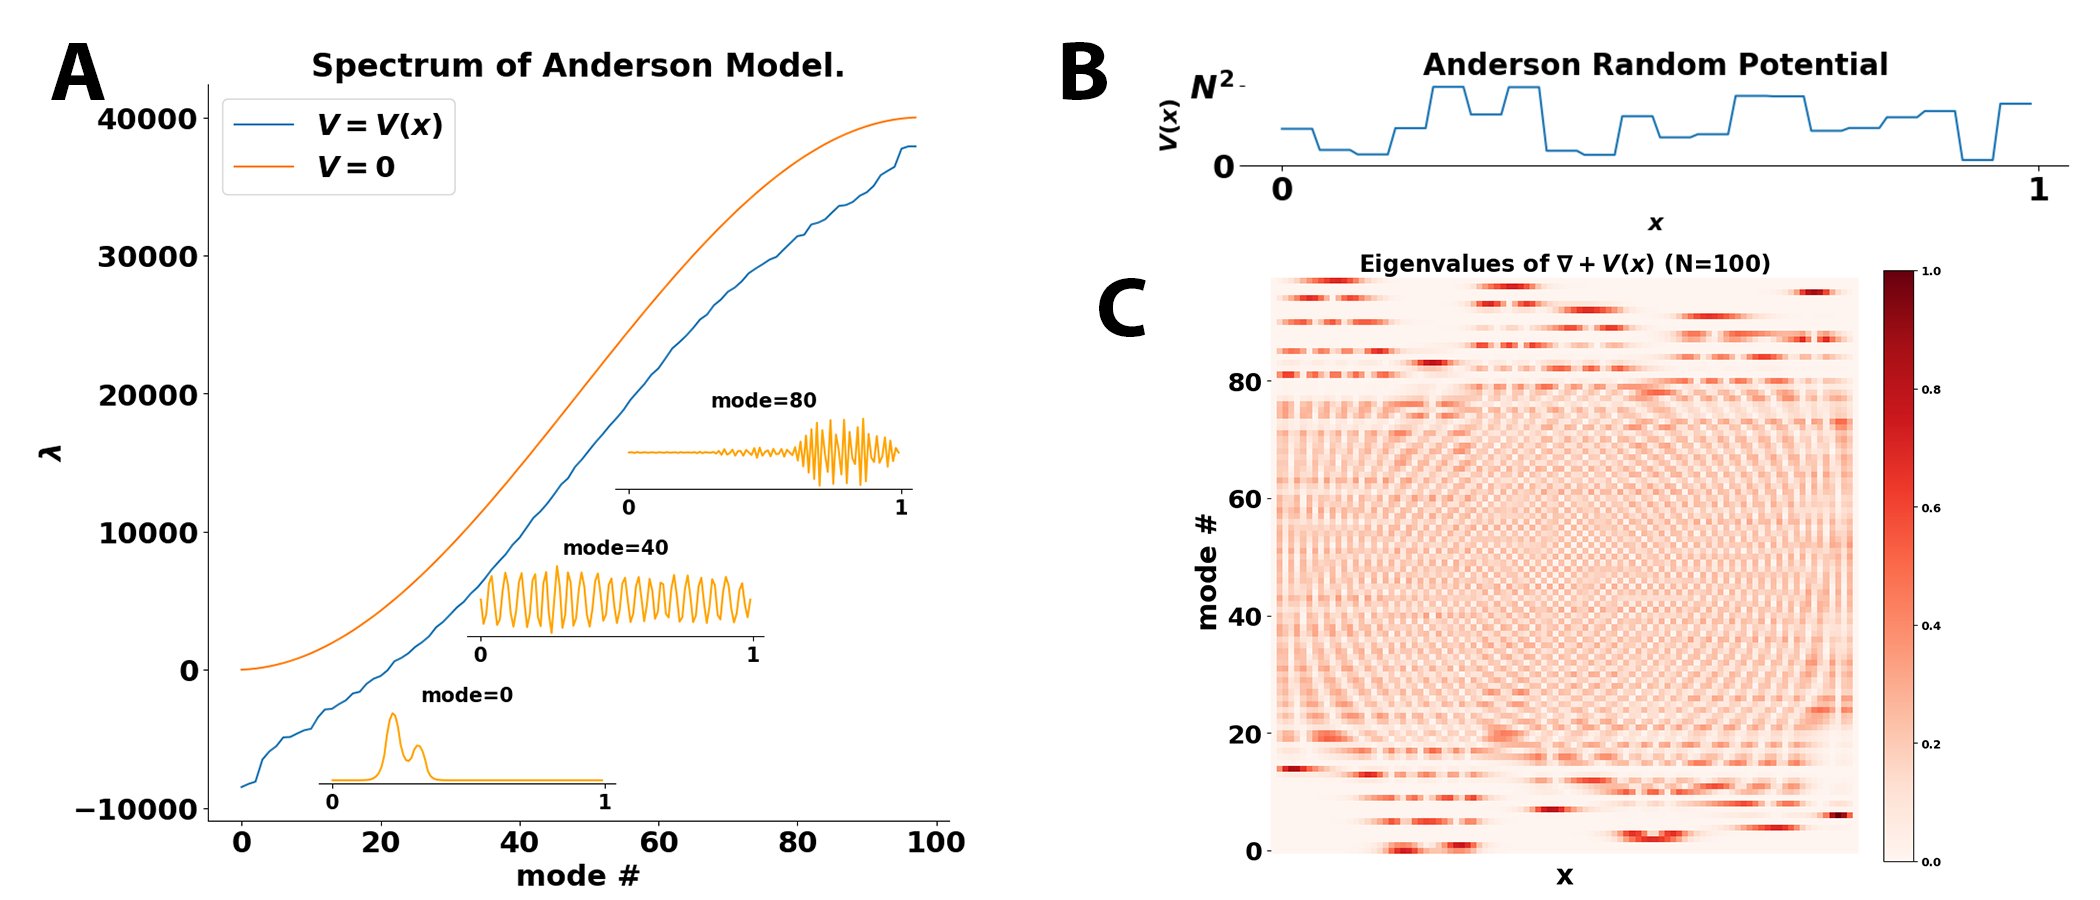
\includegraphics[width=\textwidth]{Figures/anderson_spectrum_and_eigenvector.png}
\end{center}
\caption{
	A. The spectrum of the spring system with noise $\bm{K}_0 + V$. 
	We also plot the spectrum of the ordered lattice, and observe that the potential rectifies the
	nonlinearity observed in high energy modes.
	At the same time, we observe isolation of high energy modes (also see C.)
	B. The background potential $V(x)$ consists of random values drawn from $(0, N^2)$.
	C. The eigenmodes for the system $\bm{K_0} + V$. 
	We observe localization (compact subregions of the domain in which $u_i>0$) for the low energy modes.
	However, moving above the bulk of the spectrum the eigevectors appear to re-localize, a feature not consistent with 
	Anderson's theory.
	It is hpothesized that this is a finite size effect, analagous to the nonlinear capping of the 
	frequency spectrum shown in fig. \ref{fig:lattice_spectrum}.
}
\label{fig:anderson_eigenvalues}
\end{figure}


\begin{figure}
	\begin{center}
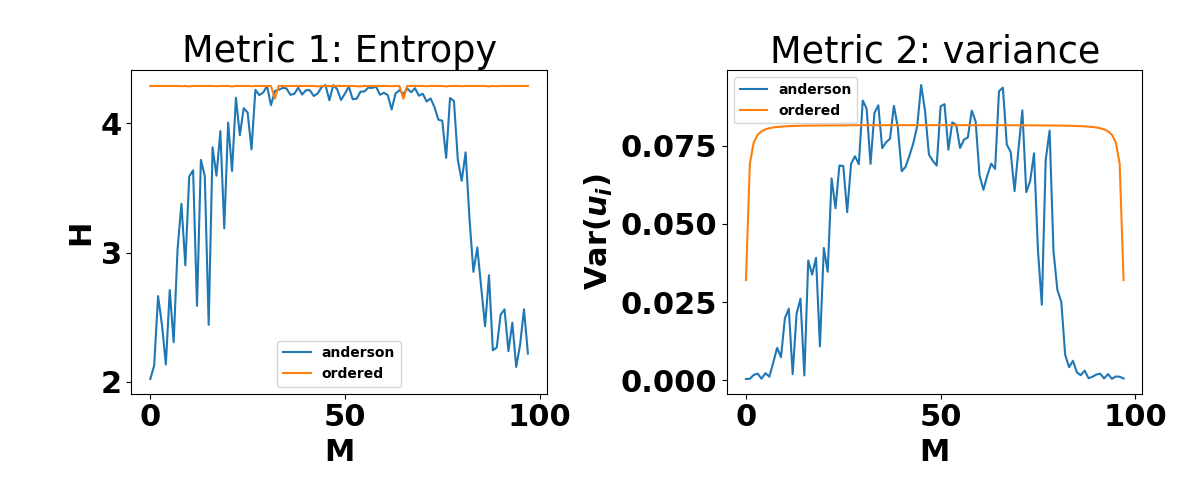
\includegraphics[width=\textwidth]{Figures/localization_metric_demo.png}
\end{center}
\caption{
	Comparison of the two localization metrics proposed in the text.
Each plot shows the metric for the representative anderson spectrum shown in \ref{fig:anderson_eigenvalues} as well as 
	for the ordered model given in \ref{fig:lattice_spectrum}. 
	Both metrics indicate that the eigenvectors for the ordered model are delocalized, while the
	eigenvectors for the anderson model are localized for small and large $M$, and delocalized 
	in the bulk of the spectrum.
	We see that the entropy displays a smoother transition into the bulk of the spectrum wheras 
	the variance metric appears to show a sharper fall off.
}
\label{fig:anderson_localization}
\end{figure}


\section{Random conenction models.}

Having validated our metrics for localization on the anderson model, we finally turn to analyze the localization in the experimental random-connection models described in the introduction.

\subsection{Finite bandwith connections.}

We first consider systems in which connections occur within a fixed range $W$ of any given node.
The connections strengths are sampled from a guassian distribution, and the final adjacency matrix is normalized such that the average force
is the same as the ordered linear model.
Explicitly, the adjacency matrix (whose ($i, j$)th enttry gives the strength of the bond between nodes $i$ and $j$ is given by \ref{eq:finite_bandwidth_adjacency}.
In this section, in addition to considering the spectrum of the corresponding stiffness matrix $K$, we also analyze the spectrum of the connectivity $A$ itself.
This is because $A$ is a \textit{Random Band Matrix (RBM)}, whose properties have been analytically studied \cite{Bourgade2018-qz}.
In particular, it is known that there is a localization/delocalization transition around $b \approx 1.4$\cite{Casati1990-ma}. 
Furthermore, it is known that the localization metric $\beta$ collapes as a function of $b\equiv \frac{W^2}{N}$, so we will use b for the plots in this section.

\begin{equation}\label{eq:finite_bandwidth_adjacency}
	A_{i,j|j\geq i} = \begin{cases}
		\mathcal{N}(0, 1) & \text{if} \left| i-j \right| \leq W \\	
		0 & \text{if} \left| i-j \right| > W 
	\end{cases}
\end{equation}

Representatives of the \textit{RBM} and \textit{RSM} matrices are plotted in \ref{fig:finite_bandwidth_K} and a sample of spectrum and eigenvectors of the \textit{RSM} are plotted in \ref{fig:finite_bandwidth_sample}.
We observe that this system has dramatically different spectral properties than either the anderson or ordered models. 
In particular, there appears to be a phase transition in which these bulk delocalized modes change into delocalized modes similar to that of a  
GOE matrix.

We study this in fig  \ref{fig:RSM_RBM_collapse}, in which we plot the order parameters for both \textit{RSM} and \textit{RBM} matrices while
varying $N$ and $W$.
Our results here for the $RBM$ match previoulsy published analytical studies, which found that the order parameter $\beta$ collapes for all $N, W$ values as a function of $b$.
We see notably different behaviour for the $RSM$ which appears to follow the $RBM$ order initially, but instead of approaching 
$GOE$ statistics (i.e. asymptotically approaching $\beta=1$), approaches some other asympotic value $0<<\alpha <1$.
Since this behaviour seems qualitatively consistent for all the $RSM$ sampled, 
suggesting that this behaviour is associated with the nonlinear construction procedure for $\bm{K}$.

\begin{figure}
\begin{center}
	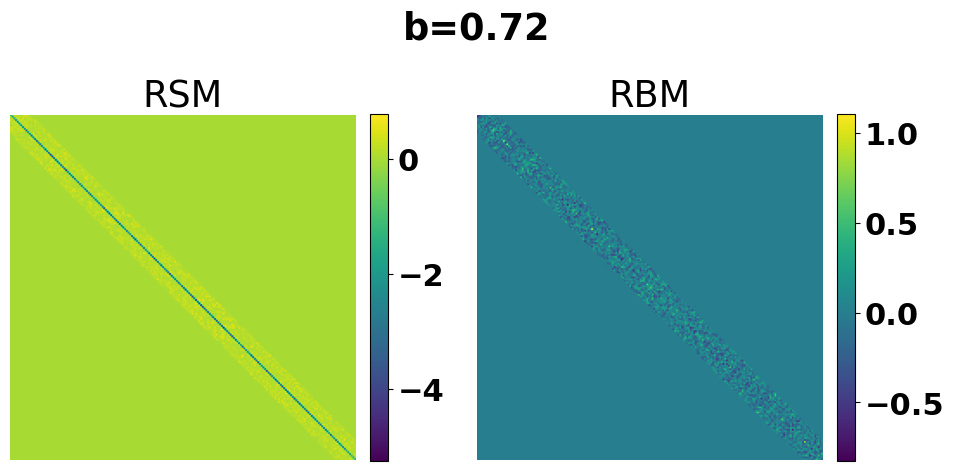
\includegraphics[width=.6\textwidth]{Figures/rsm_rbm_example.png}
\end{center}
\caption{Representative matrices of the RBM and RSM class. 
Note that the essential difference is that the RSM is positive everywhere outside of the diagonal, and negative on the diagonal.
Furthermore, by construction, the sum of the off-diagional elements in each row is equal to negative the corresponding diagonal value (this is required by to the symmetry of forces between nodes).}
\label{fig:finite_bandwidth_K}
\end{figure}


\begin{figure}
\begin{center}
	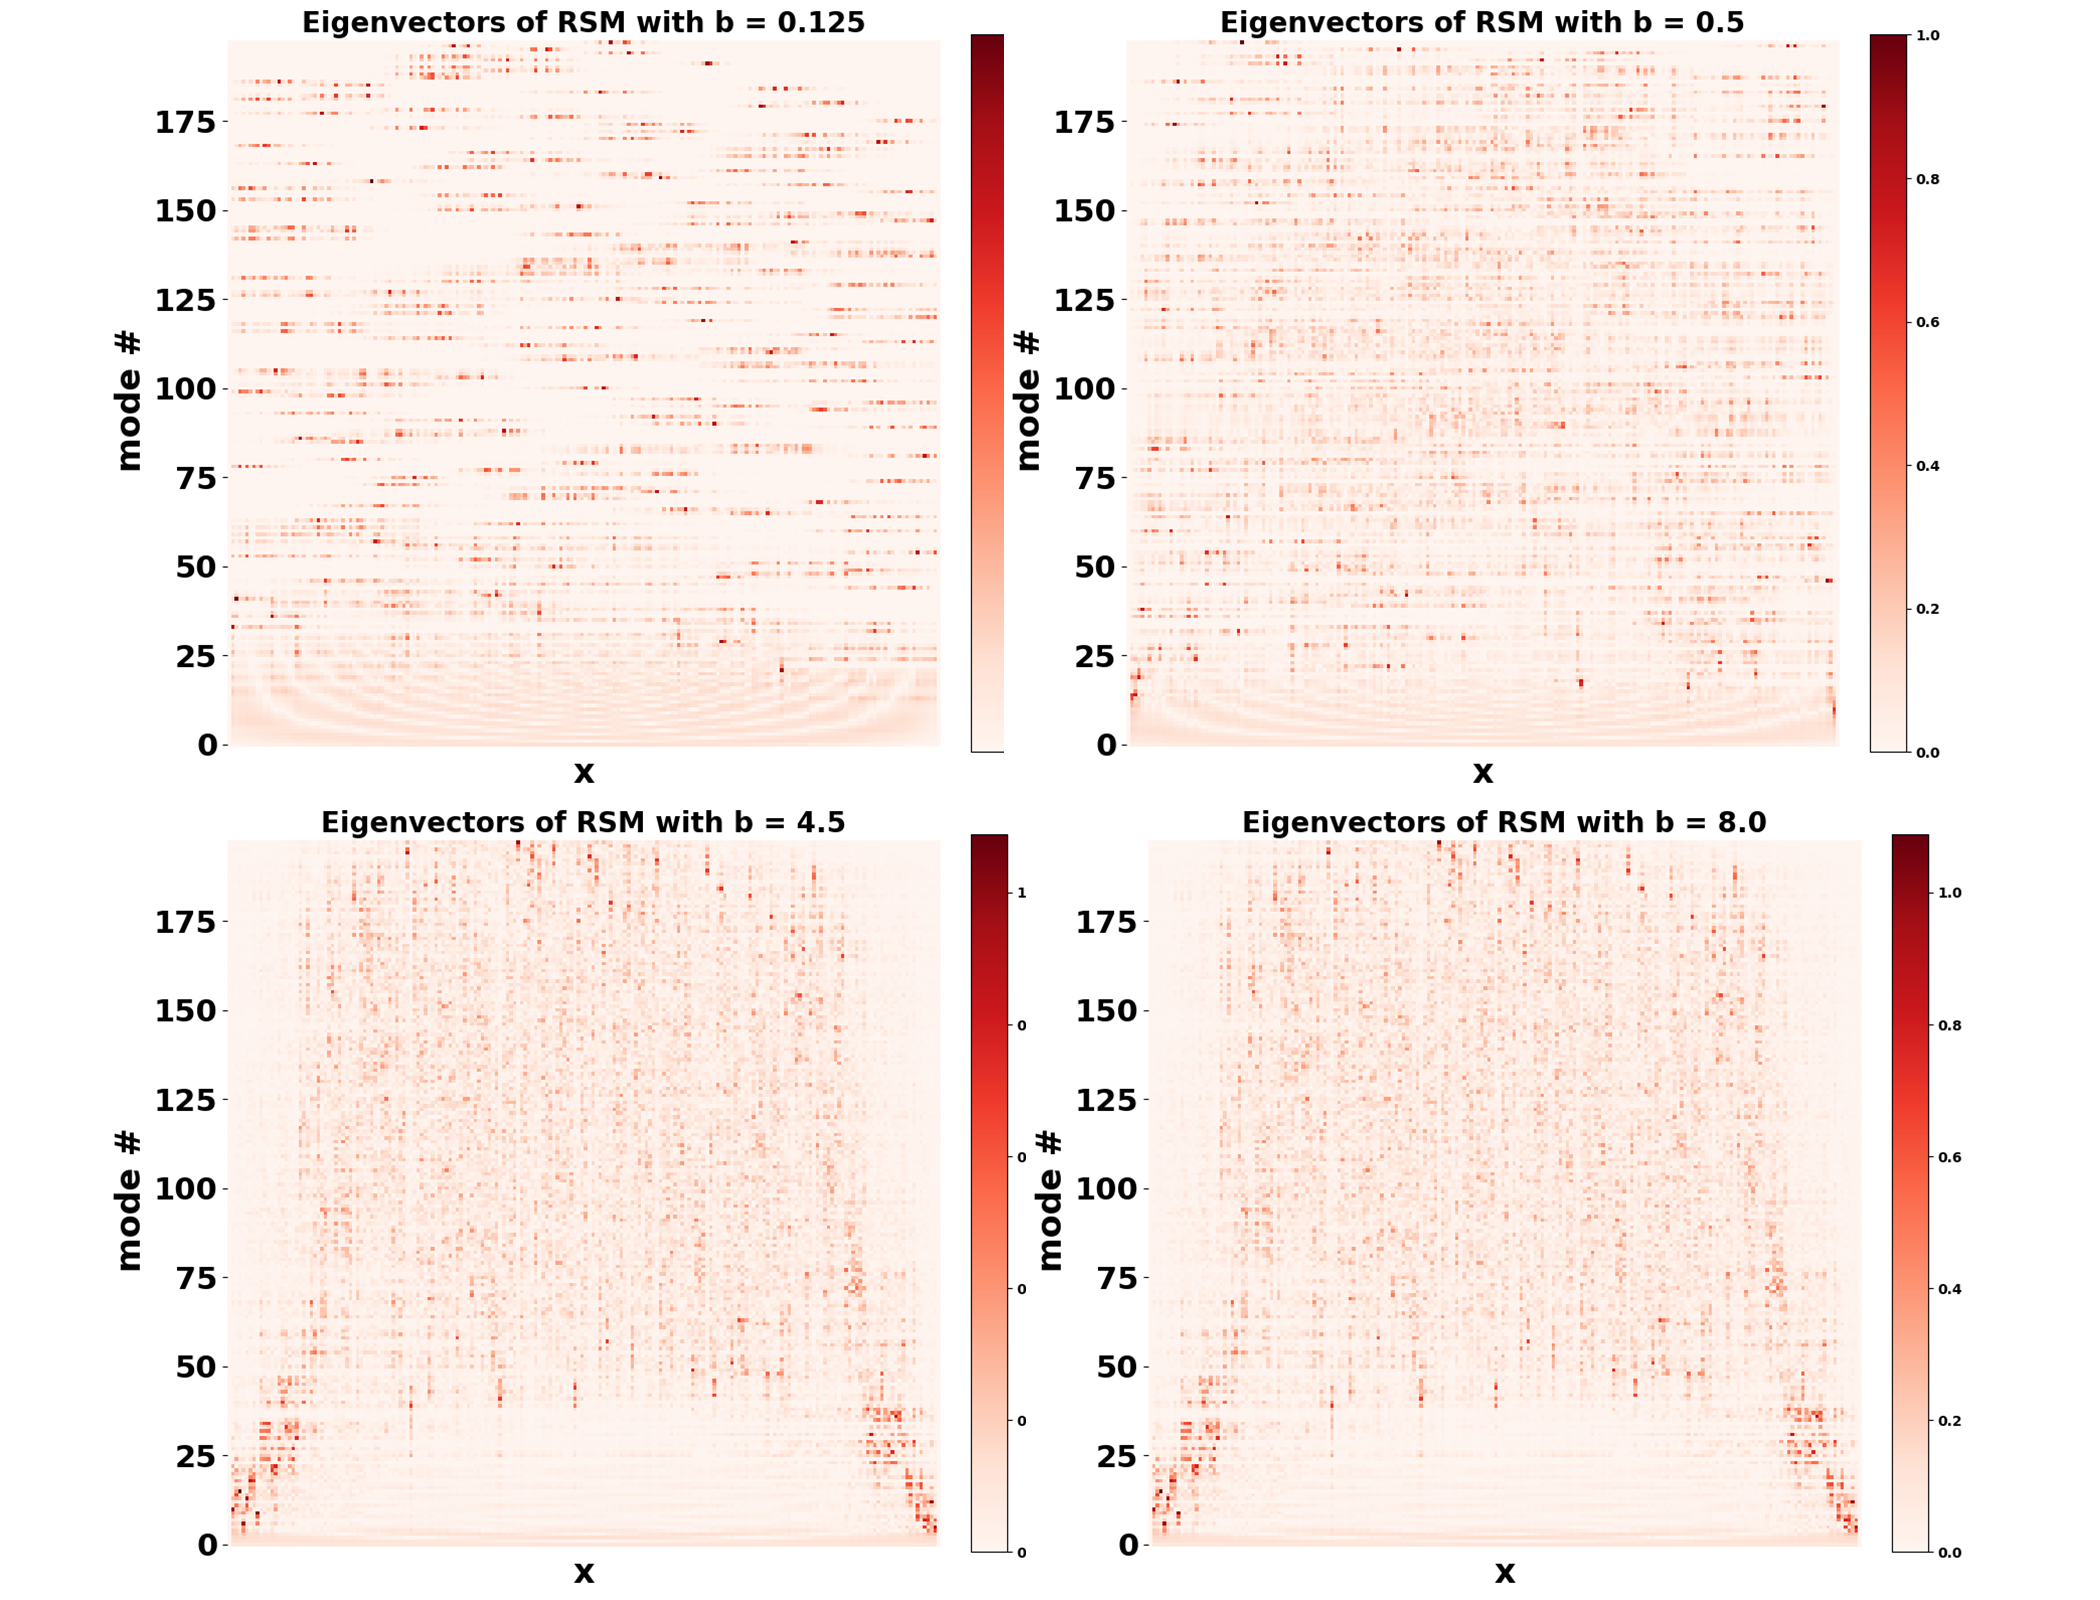
\includegraphics[width=\textwidth]{Figures/RSM_eigenvectors.png}
\end{center}
\caption{Sample of 4 eigenvector plots for RSM with various values of $b$. 
(N=200). for small $b$ we observe a set of low frequency modes evocative of the delocalized modes of the ordered chain. 
In addition, at small $b$ one can see a high degree of localization throughout the bulk of the spectrum, notably different from the
anderson-type localization previously encountered.
As $b$ (or equivalently, $W$) increases, we observe that the number of these ``ordered'' modes decreases and the system appears to contain
primarily delocalized random eigenvectors.}
\label{fig:finite_bandwidth_sample}
\end{figure}

\begin{figure}
\begin{center}
	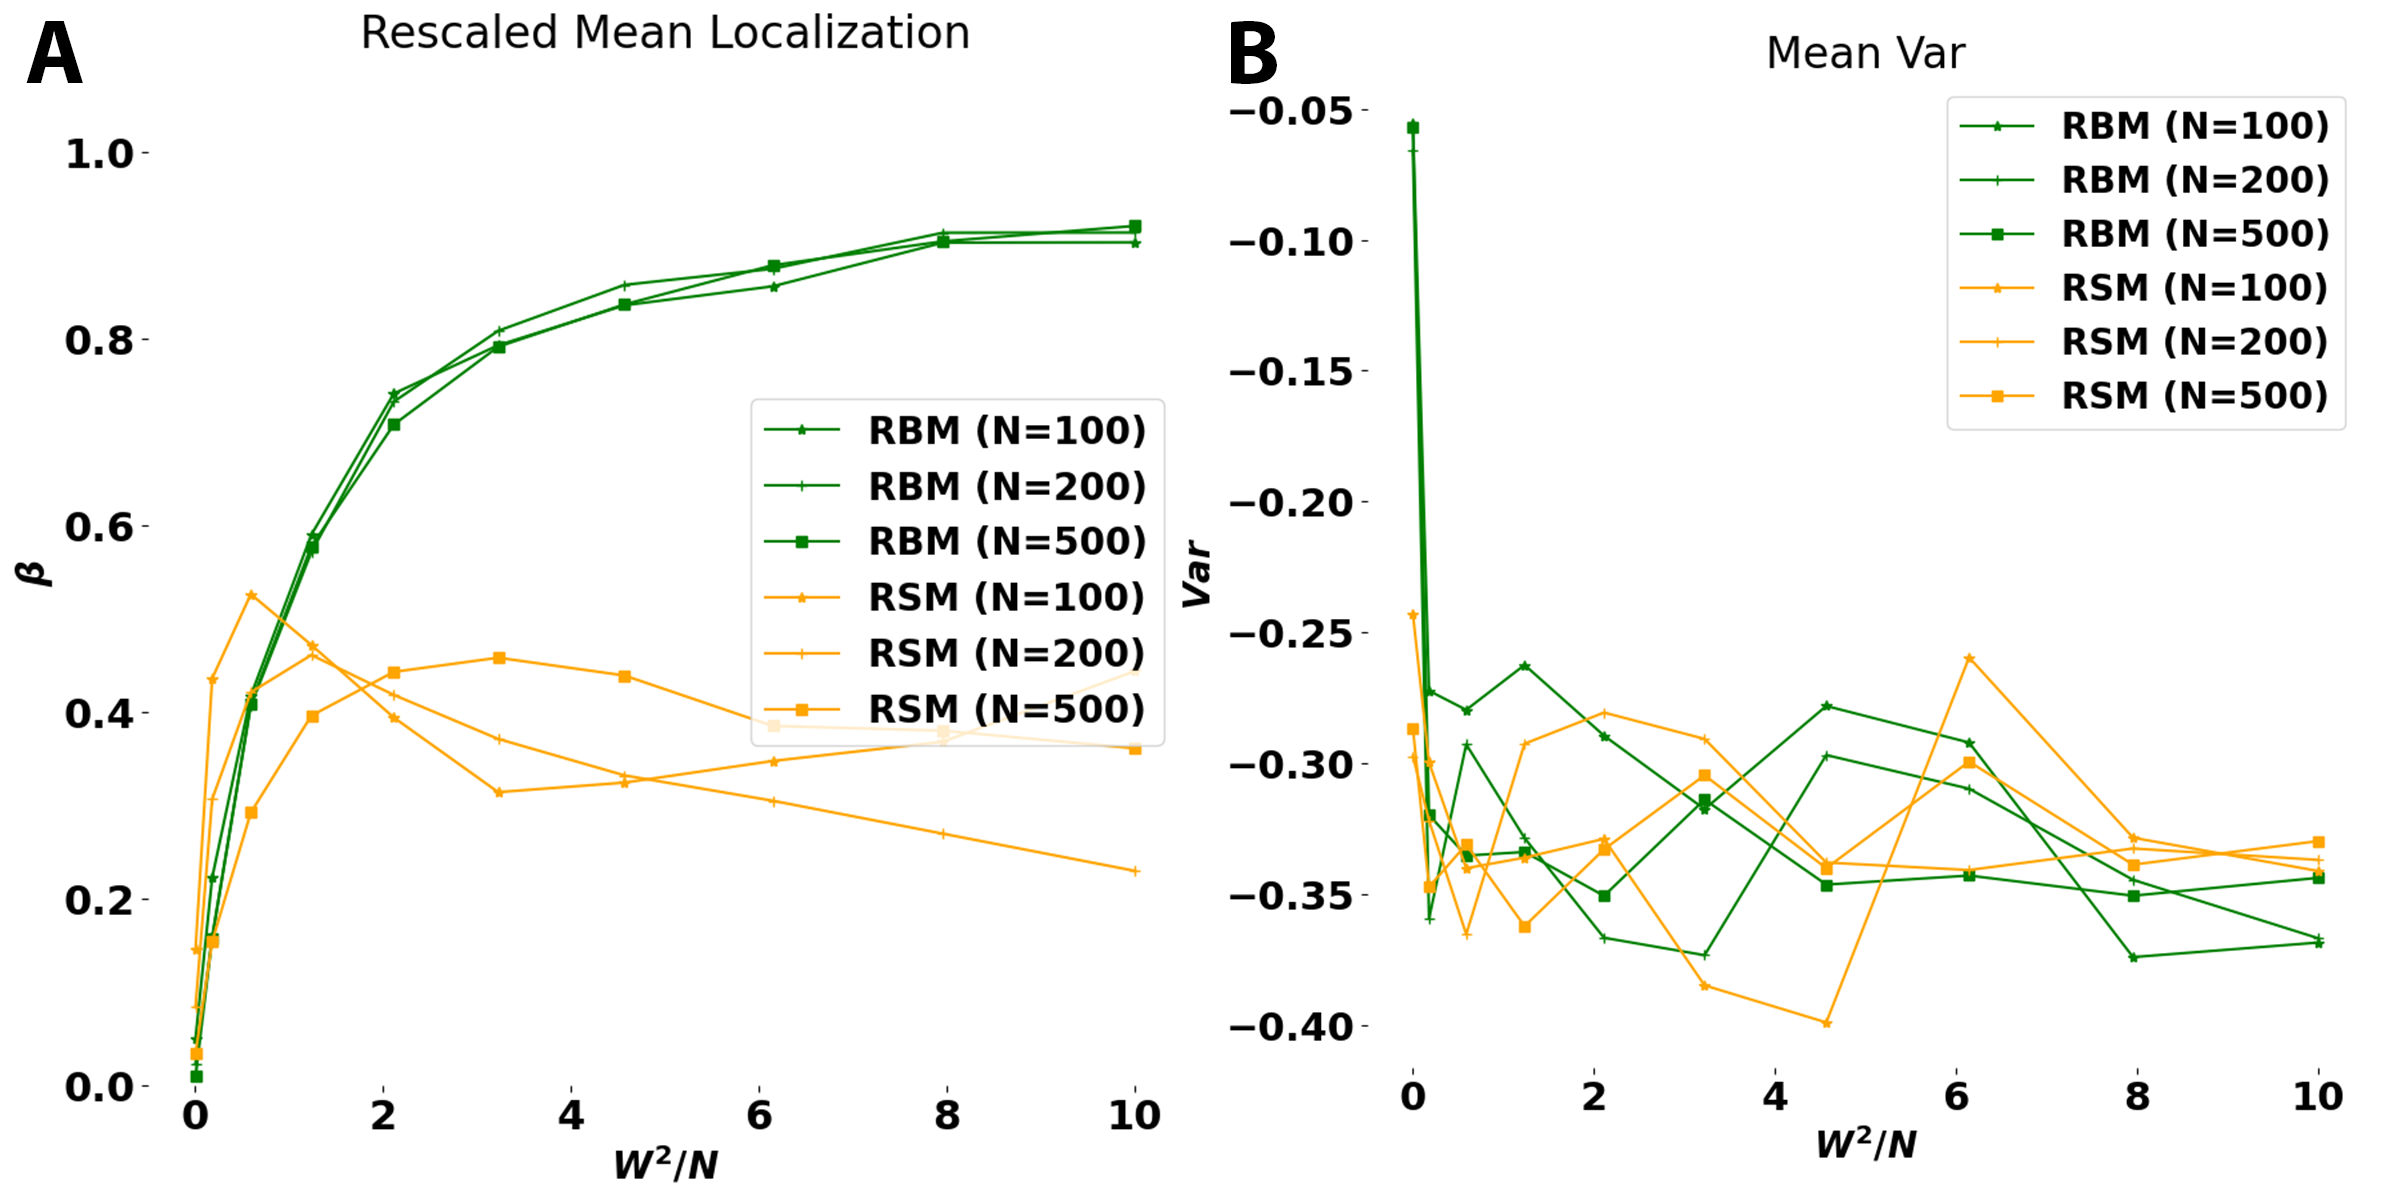
\includegraphics[width=\textwidth]{Figures/RSM_RBM_localization_final.png}
\end{center}
\caption{
A. Plot of the entropy order paramter ($\beta$) for a sample of RBM and RSM matrices. 
We observe the localization of the RSM has a non-monotonic dependence on $b$. 
This could suggest either that $b$ is not the appropriate scaling, or be due to the 
nonlinear construction of the stiffness matrix.
B., Plot of the mean eigenvector variance for the same RBM and RSM matrices. 
It appears this metric (when averaged over the entire ensemble of eigenvectors)
is much less suited to detecting the type of localization observed for RSM matrices.}
\label{fig:RSM_RBM_collapse}
\end{figure}



\subsection{Long range perturbation.}%
\label{sec:sparse}

Finally, we consider the spectrum of matrices with sparse long-range interactions.
We construct the connectivity matrix $A$ as given by \ref{eq:random_sparse}.
In order to differentiate the resulting matrices from those of the preciding section we will refer to these as \textit{Sparse Random Stiffness Matrices (SRSM)} and the corresponding random matrix as \textit{Sparse Random Matrices (SRM)}.
In eq \ref{eq:random_sparse} $X$ represents a contribution from random bonds, while $\theta$ controls the SNR of the
underlying laplacian (ordered chain) relative to the long range interactions.
The long range interactions are sampled from a GOE distribution, and we supplement an average of $n$ bonds per mass, following a binomial distribution evaluated for each pair of nodes independently.

We again plot a sample of representative eigenvectors in fig \ref{fig:sparse_springs_example}.
We observe that modes are localized even for small values of $z$ and large values of $\theta$ throughout the bulk of the spectrum.
We also plot the localization parameter $\beta$ for this

\begin{equation}\label{eq:random_sparse}
	\boldsymbol{A} = \theta \nabla + X
\end{equation}

\begin{figure}
\begin{center}
	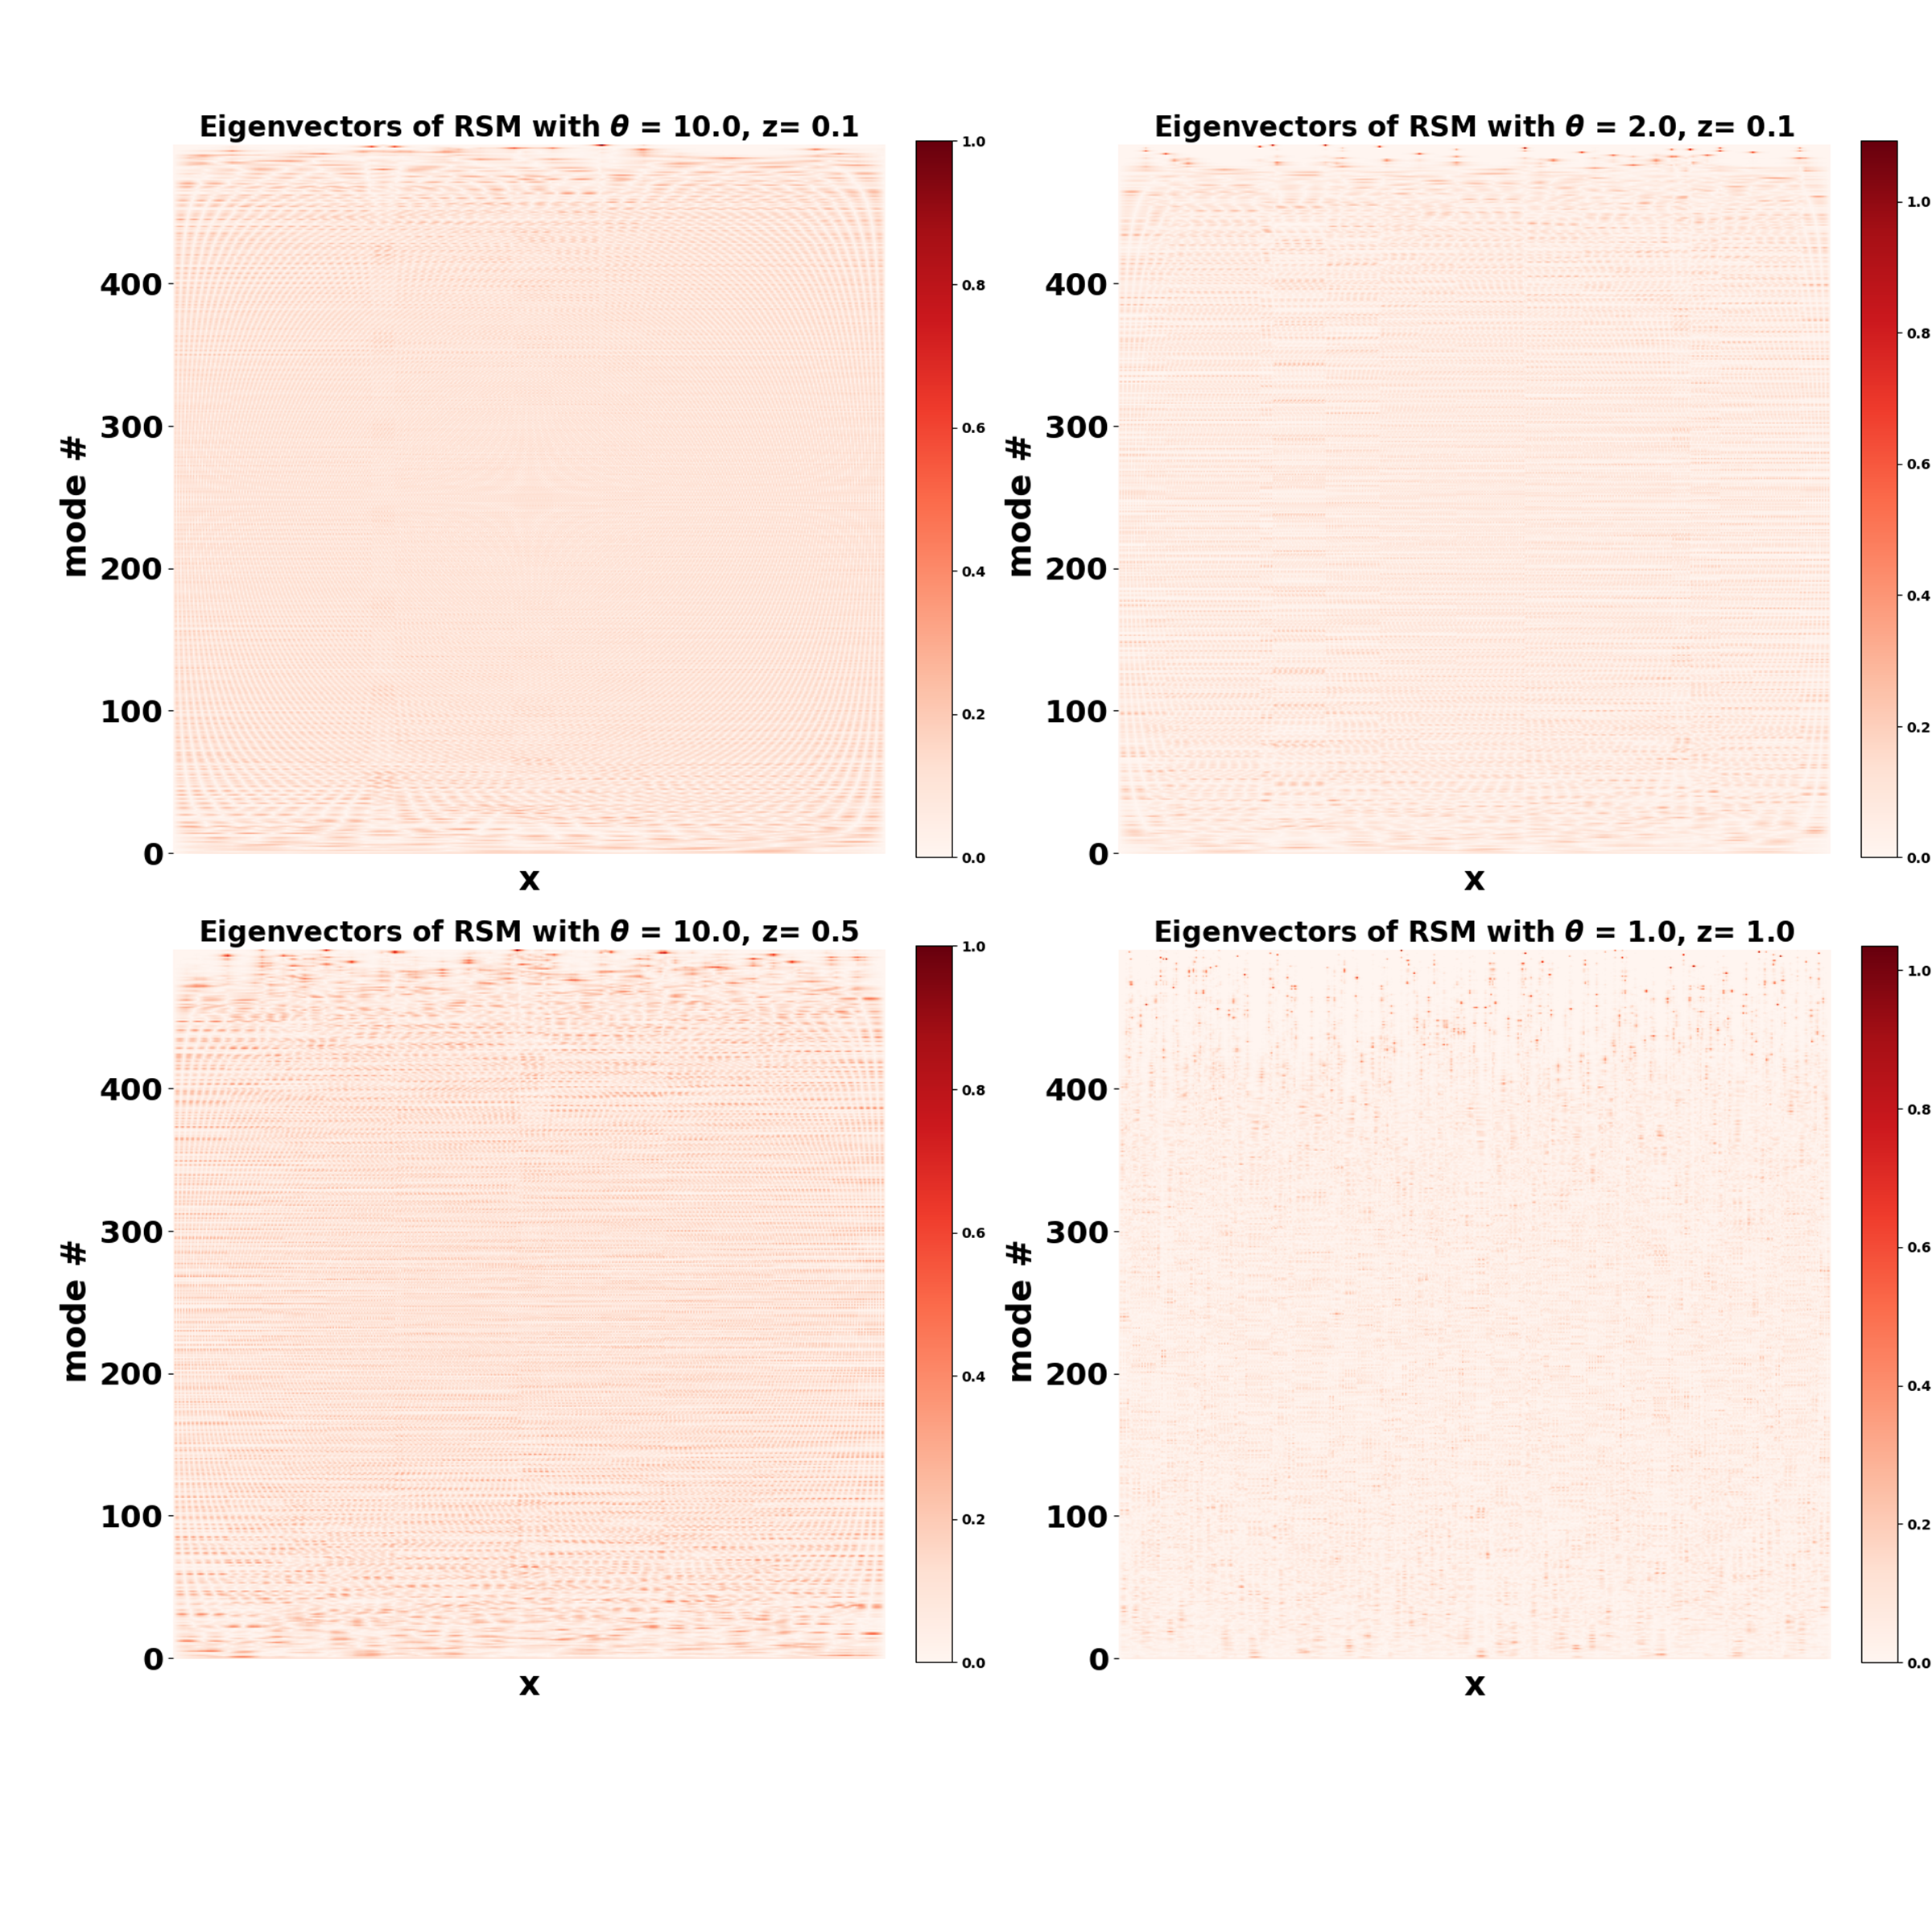
\includegraphics[width=\textwidth]{Figures/sparse_eigenvectors.png}
\end{center}
\caption{Sample of 4 eigenvector plots for the sparese RSM with various values of $z$ and $\theta$. }
\label{fig:sparse_springs_example}
\end{figure}


\begin{figure}
\begin{center}
	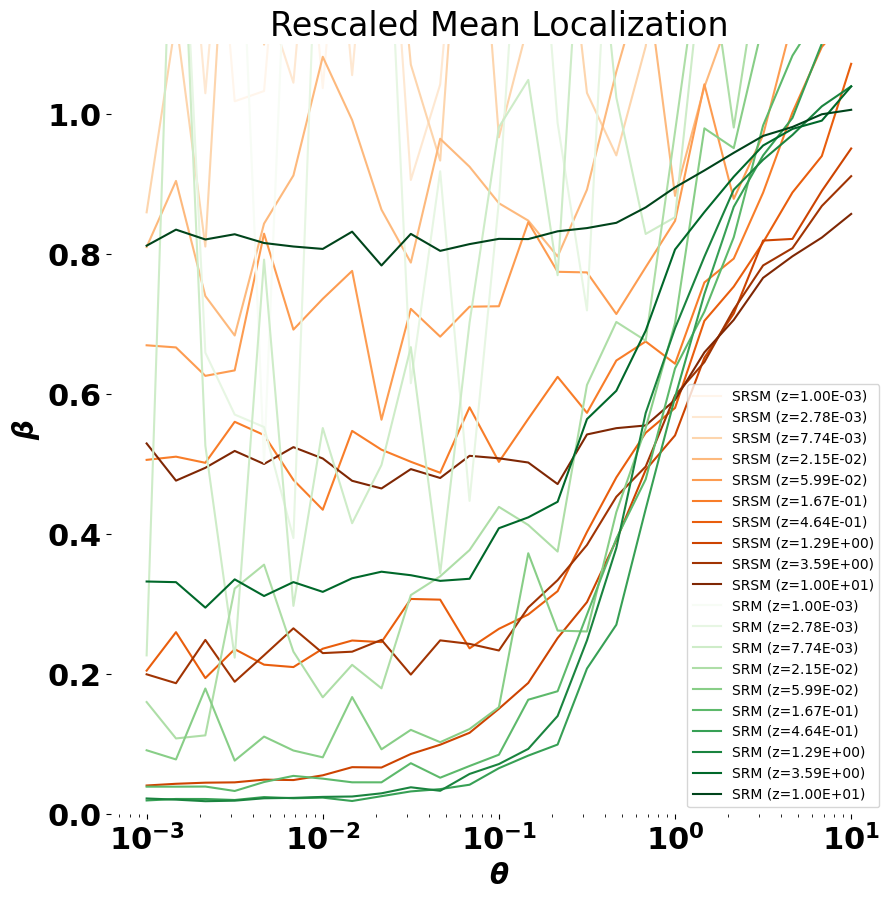
\includegraphics[width=\textwidth]{Figures/sparse_RSM_RBM_localization.png}
\end{center}
\caption{
A. Plot of the entropy order paramter ($\beta$) for a sample of sparse SRM and SRSM matrices. 
We do not capture any obvious scaling relationships here, although there may be a limiting curve as $z\rightarrow N$ for the $SRM$.
It also appears that the degree of localization is less for the same $z$ and $\theta$ values for the \textit{SRSM} compared to the \textit{SRM}.
However, localization appears to be preserved for larger values of $z$ at the same $\theta$ value for the \textit{SRSM} compared to \textit{SRM}.
}
\label{fig:sparse_RSM_RBM_collapse}
\end{figure}


\section{Future Work}

This empirical computational study suggests several potentially exciting avenues for future research. These include:

\begin{itemize}
	\item Understanding the impact of finite-size effects in disordered spring network systems. 
		As was observed both for the anderson and experimental random models, there was a high degree of localization 
		in a manner that appears suggestively symmetric with the low energy localization.
	\item Analytical description of the localization curves for the local \textit{RSM} models, and in particular, a prediction for the divergence from the \textit{BSM} models.
	\item Redo empirical studies with larger sample sizes and exhaustive parameter sweeps. Most of the data presented in this paper represents a single sample into the respective parameter regime, and figures like \ref{fig:sparse_RSM_RBM_collapse} would benefit from larger statistics.
	\item Find a scaling parameter for both the \textit{SRSM} and \textit{SRM} models.
	\item For the simplest systems, scale $k_{i,j}$ as a function of the bond length. 
		This is more representative of physical elastic materials (shorter springs have higher stiffness) and has also been shown to liead to interesting equilibrium behavior \cite{Adam2022-qd}.
\end{itemize}

\section{Code}

All code for the simulations in this paper can be found at \href{https://github.com/Noahyt/AM254}{https://github.com/Noahyt/AM254}.

\bibliography{references}
\bibliographystyle{plainnat} % Needed for \cite.


\end{document}
